\documentclass{article}

% formatting
\usepackage[utf8]{inputenc} % allow utf-8 input
\usepackage[T1]{fontenc} % use 8-bit T1 fonts  (allows for direct use of ö,ü,etc.)

% math typesetting
\usepackage{amsmath}
\usepackage{amssymb}
\usepackage{amsfonts}

% maths definitions, theorems, etc.
\usepackage{amsthm}

% color
\usepackage{color}
\usepackage{xcolor}

% layout
\usepackage{layout}
\usepackage{lipsum}

% cross-referencing and hyperlinks
\usepackage{hyperref}
\usepackage{url}
\usepackage{doi}

% figures
\usepackage{graphicx}
\usepackage{subfig}
\usepackage{wrapfig}

% tables
\usepackage{booktabs}
\usepackage{multirow}
\usepackage{caption} 
\usepackage{float}

% enumeration
\usepackage{enumitem}

% embedding pages
\usepackage{pdfpages}

% multi-line comments
\usepackage{comment}

% landscape orientation
\usepackage{rotating}
\usepackage{pdflscape}

% Gantt charts
\usepackage{pgfgantt}

% footnotes
\usepackage{footnote}

% code
\usepackage{listings}

% matrices and tables
\usepackage{nicematrix}
\usepackage{varwidth}
% \usepackage{tabularx} do not load package tabularx, instead use package nicematrix

% document structure
\setcounter{secnumdepth}{5} % enable numbered sub-sub-sections etc.

% custom header size
\usepackage{titlesec}

% customized references (make "Figure 1" a link, not just "1")
\usepackage[capitalise, nameinlink]{cleveref}

% customized frames around text etc.
\usepackage{mdframed}

% tikz
\usepackage{tikz}

% calligraphy
\usepackage{calligra}

% chemical formulas
\usepackage{chemformula}
% column layout
\usepackage{multicol}
\setlength{\columnsep}{0.75cm}

% paragraphs
\usepackage[skip=0.5\baselineskip]{parskip}

% geometry
\usepackage[
    margin = 3cm,
    top = 3cm,
    bottom = 3cm
]{geometry}

% header size
\titleformat*{\section}{\large\bfseries}%{\thesection.}{\hspace{0cm}}{}
\titleformat*{\subsection}{\normalsize\bfseries}%{\thesection.}{\hspace{0cm}}{}
\titleformat*{\subsubsection}{\normalsize\bfseries}
\titleformat*{\paragraph}{\normalsize\bfseries}
\titleformat*{\subparagraph}{\normalsize\bfseries}

% custom headers
\usepackage{fancyhdr}
\pagestyle{fancy} % custom headers and footers
\setlength{\headheight}{15pt} % height of header
\setlength{\headsep}{10pt} % separation between header and main text

\usepackage[
    backend=biber,
    style=ieee
]{biblatex}
\addbibresource{references.bib}
% show DOI URL (https://doi.org/XXX.XXXXX.XXXX), instead of publisher URL (https://springer.com/XXXX)
% cf. https://tex.stackexchange.com/a/616241
\DeclareSourcemap{
  \maps[datatype = bibtex]{
    \map{
      \step[notfield = keywords, final]
      \step[fieldsource = doi, final]
      \step[fieldset = url, null]
    }
    \map{
      \step[fieldsource = keywords, notmatch = \regexp{\bprimary\b}, final]
      \step[fieldsource = doi, final]
      \step[fieldset = url, null]
    }
  }
}
\AtEveryBibitem{
    \clearfield{urlyear}
    \clearfield{urlmonth}
}

%%%%%%%%%%%%%%%%%%%%%%%%%%%%%%%%%%%%%%%%%%%%%%%%%%%%%%%%%%%%%%%%%%%%%

% document metadata
\title{Proposal for a Summer Academy \protect\\ of the Swiss Study Foundation}
\author{Michael P. Weinold$^1$, Philippe Schultheiss$^1$, Mark C. Ballandies$^2$}
\date{
    $^1$Schweizerische Studienstiftung \\
    $^2$Studienstiftung des Deutschen Volkes \\[3mm]
    October 2023
}

%%%%%%%%%%%%%%%%%%%%%%%%%%%%%%%%%%%%%%%%%%%%%%%%%%%%%%%%%%%%%%%%%%%%%

\begin{document}

\maketitle

\section*{\centering Authors}

\textbf{\textit{Michael P. Weinold}} (born 1995 in Innsbruck, Austria) is a doctoral researcher at ETH Zurich and Paul Scherrer Institute. His research is focused on accelerating innovation in clean-energy technologies. He has a  background in engineering physics.

\textbf{\textit{Philippe Schultheiss}} (born 1984 in Basel, Switzerland) was formally trained in philosophy and economics at the universities of Basel and Fribourg. He presently works as an independent consultant, coach and author. At the same time, he is the President of the Parliament of Europe's largest church community since 2020, alongside pursuing theology studies at the University of Zurich since fall 2021. 

\textbf{\textit{Mark C. Ballandies}} (born 1991 in Burgwedel, Germany) is a postdoctoral researcher at the Department of Computational Social Sciences at ETH Zurich. His research is focused on utilising emerging digital technologies to promote more participatory forms of democracy. He has a background in Computational Science and Engineering.

\textit{"[Architecture] (...) is the most overweening of the arts, and the one that least lets us alone. A gallery we can't walk out of, a book we can't close, an art we can't even turn our back on because it is there facing us on the other side of the street as well (...)} - British poet Blake Morrison in "Lords of glass, steel and concrete" \cite{morrison_lords_1982}

\clearpage
\tableofcontents

\section{\centering Abstract}

\begin{minipage}{0.55\textwidth}
    We must reduce global carbon emissions dramatically. The construction sector is responsible for XX\% of annual global carbon emissions. In Switzerland, it accounts for XX\% of carbon emissions (including imported carbon). This number is expected to increase to XX\% in 2050, due to strong immigration.
    
    What is more, the construction sector is notoriously difficult to decarbonise. Together with certain heavy industry sectors and aviation, it is classified as a "hard to abate" sector.
    
    Work is ongoing on decreasing the carbon footprint of building during the construction phase and during the use phase. This includes novel methods for cement, concrete and steel production or the increasing digitisation of buildings ("smart home"). However, there are currently no efforts to increase the lifetime of buildings. In Switzerland, like in the surrounding EU countries, average building lifetime is around 50 years only.
    
    The carbon emissions incurred during new construction of a building vs the refurbishment can be recouped over a period of between XX-XX years. Studies exist for the nordic countries, where the energy cost of non-refurbished buildings is highest. Average building lifetimes are between 50 years (France, with source) and 60 years (Switzerland, with source).
    
    Despite efforts to improve recycling in construction, recycling rate of modern building materials (steel, concrete, glass) remains low (check for source).
    
    [Figure from Crawford on cumulative embodied energy]
    
    At the same time, changing use requirements meet the modernist credo "form follows function". Changing family structures mean that apartments can be ever more compact.
    
    All this amounts to large scale new construction, the majority of which is in the 'modernist' or contemporary style.
    
    Every poll to date has shown that this style is at the very least moderately unpopular with people. Empirical evidence is mounting, thereby providing proof for something that has been well-known to the general public for a long time: "Why is the Modern World So Ugly?" (Alain de Boton)

\end{minipage}\hspace{15mm}
\begin{minipage}{0.2\textwidth}
    \begin{figure}[H]
    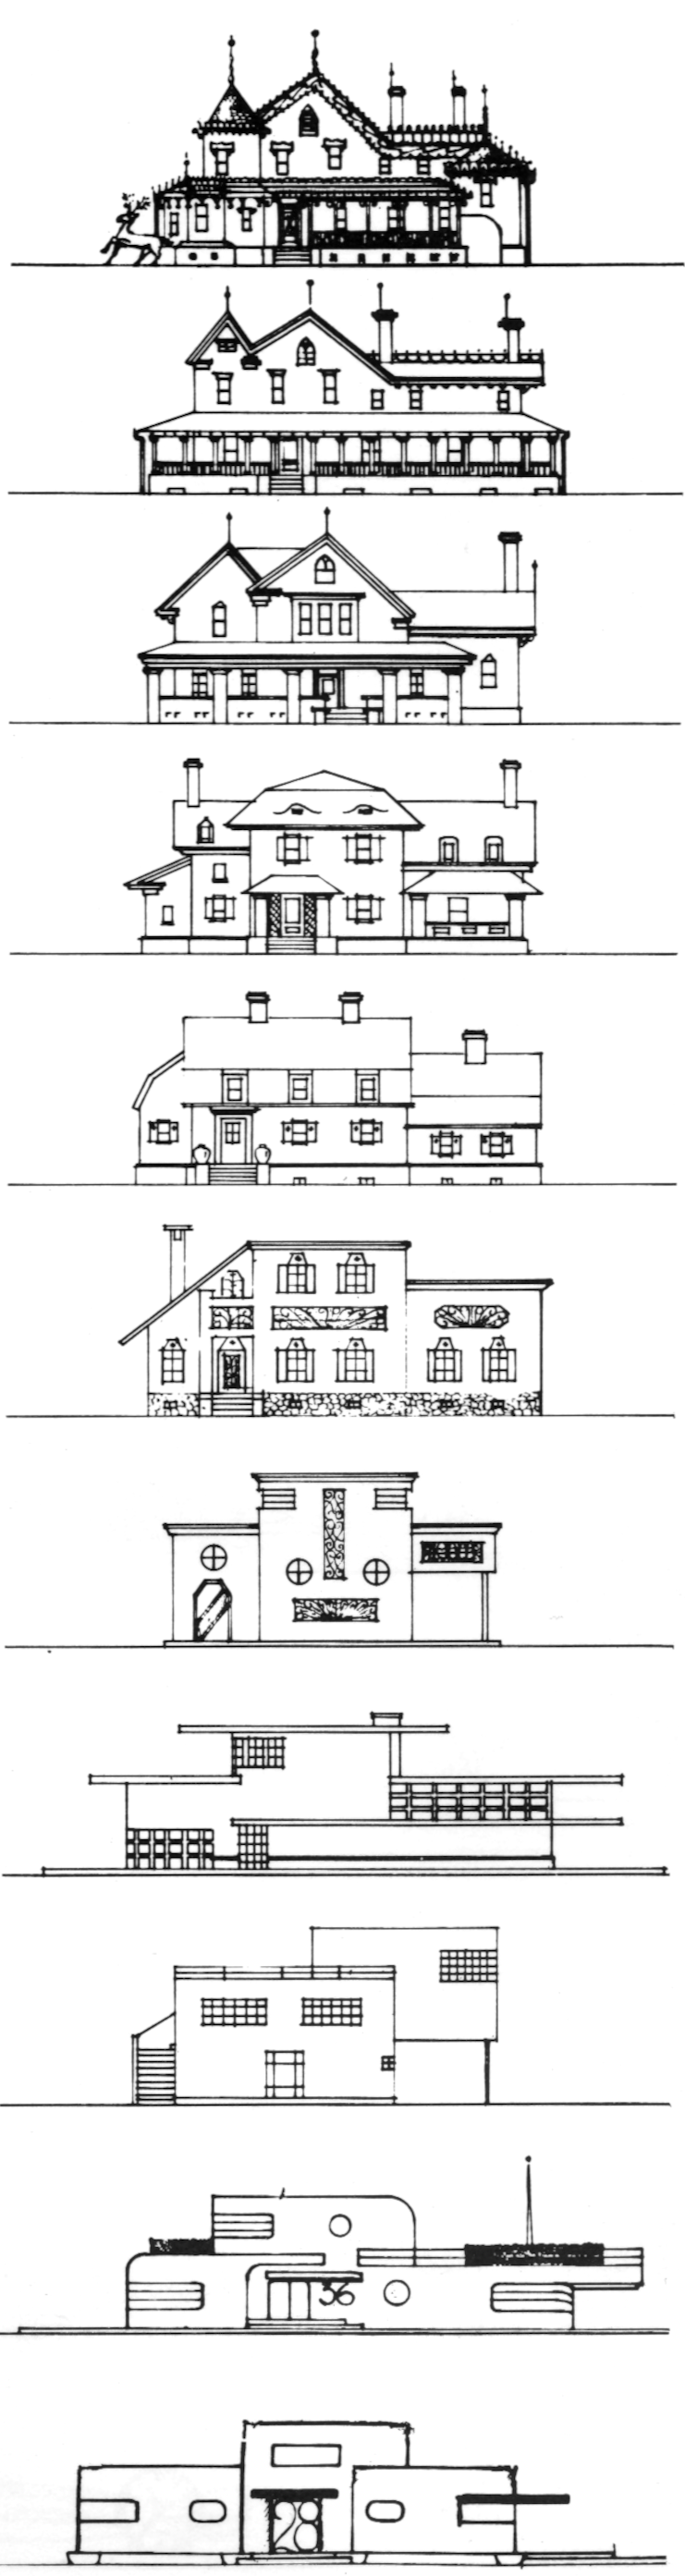
\includegraphics[width=50mm]{./figures/loewy_architecture.png}
    \caption{
        "Design Evolution 1930" by French-born American industrial designer Raymond Loewy \cite{loewy_industrial_1979}
    }
    \label{fig:loewy}
    \end{figure}
\end{minipage}

\clearpage
\section{Context}

\section{Construction and Climate Change}

\section{Construction and Aesthetics}

Modern architecture is always ugly. Nonetheless, we limit our discussion to buildings of a representative nature. We exclude housing (eg. apartment complexes) to avoid:

\section{Proposed Agenda}

\section{Proposed Speakers}

\section{Scattered Thoughts}

Architects have been publicly calling for the public to be re-educated to appreciate their brutalist/modernist designs. (eg. the architects that build the Triemli Tower).

Some potential pathways to decarbonizing the economy are difficult for technical and political reasons. This includes "flying less", "reducing personal mobility", etc.
However, some aspects should be really simple: "don't design houses for a 50 year lifetime"

\section{Sustainability}


\clearpage
\section{"Why is the modern world so ugly?}

\subsection{Mounting Empirical Evidence}

As we have seen illustrated in the proclamations of Corbusier and XXX, "Taste is subjective" (and we must take part in) has always been the the refuge of modernists. Corbusier said that the public had to be re-educated, and others have wondered about the vulgarity of designs for the public and asked whether architects should take these architectural tastes seriously.

\subsection{A matter of taste?}

\subsection{Re-educating the general public}

In fact, we can observe that there is a kind of self-propagating effect: architectural prizes are given out only by architects. There is no 'public vote'. The contempt with which architects have treated the public is by no means covert. This is perhaps best exemplified by the reaction of Rudolf Guyer, who in 1955 designed a high-rise residential apartment in souther Zurich. When the building was voted "Switzerland's ugiest building" in 2018 by readers of the daily newspaper \textit{20 Minuten}, he declared:

\textit{"Dass Laien das Gebäude hässlich finden, ist mir egal. Hauptsache, den anderen Architekten gefällt es."} (en.: I don't care that laypeople find the building ugly. The main thing is that the other architects like it) 



\begin{figure}[ht!]
    \centering
    \subfloat{{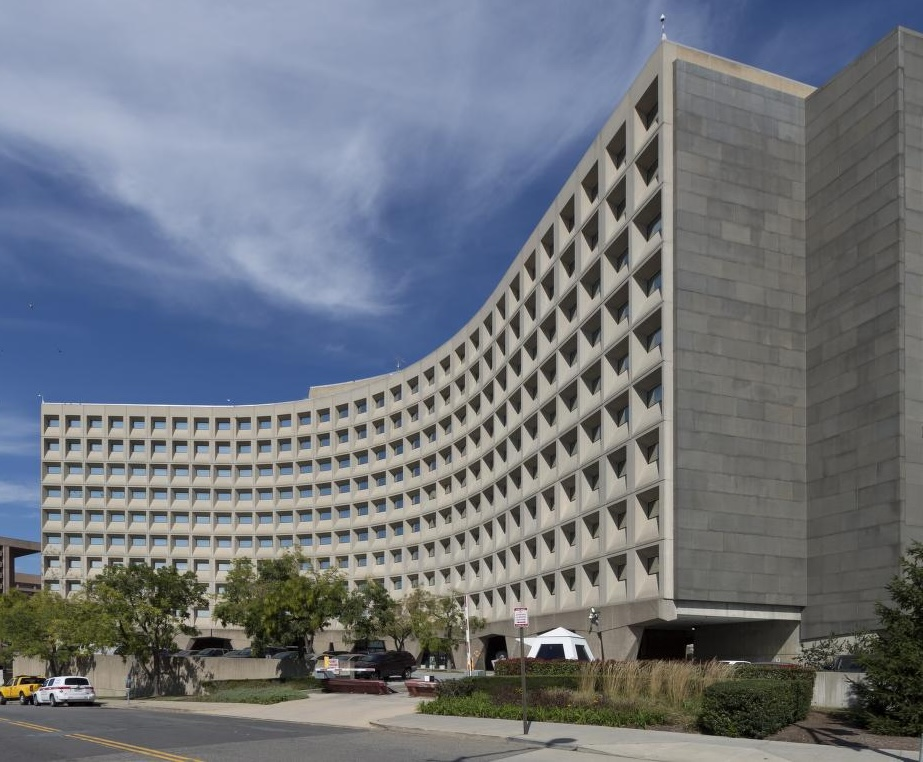
\includegraphics[height=5cm]{figures/us_gov_modernist_1.jpg} }}
    \subfloat{{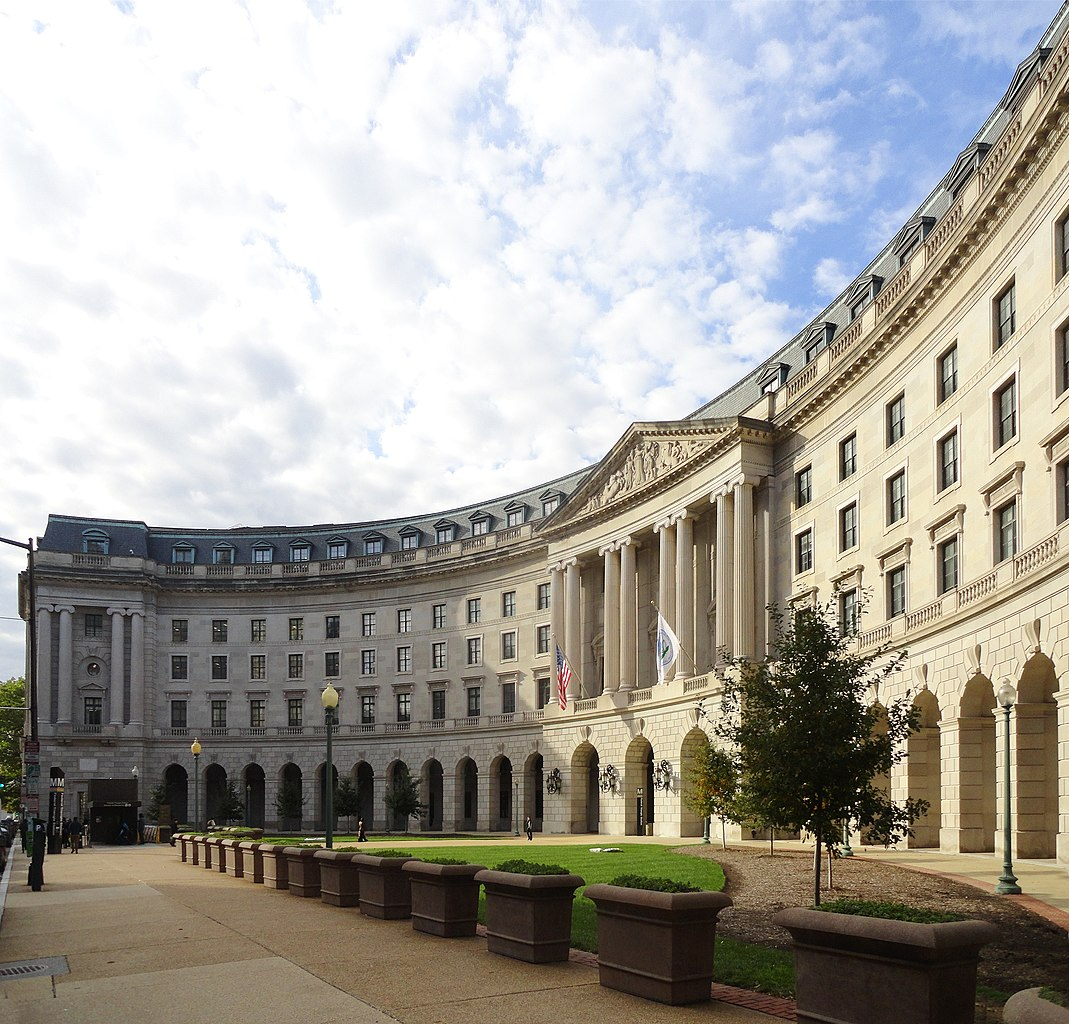
\includegraphics[height=5cm]{figures/us_gov_traditional_1.jpg} }}
    \caption{Left: The Robert C. Weaver Federal Building on 7th Street SW in Washington, D.C., designed in 1965 by Marcel Breuer. It presently serves as United States Department of Housing and Urban Development. The irony is not lost on the authors. \cite{highsmith_robert_2012}. Left: The William Jefferson Clinton Federal Building on Pennsylvania Avenue in Washington, D.C., designed in 1934 by William Adams Delano and Chester Holmes Aldrich \cite{wikimedia_commons_user_moreau1_epa_2018}. It presently serves as the headquarters of the Environmental Protection Agency. Images of this nature formed the core part of the 2020 American poll on architectural preferences \cite{noauthor_americans_2020}. All image pairs presented showed images of similar shape and purpose, thereby accounting for major non-aesthetic considerations.}
    \label{fig:federal_buildings}
\end{figure}

\begin{figure}[ht!]
    \centering
    \subfloat{{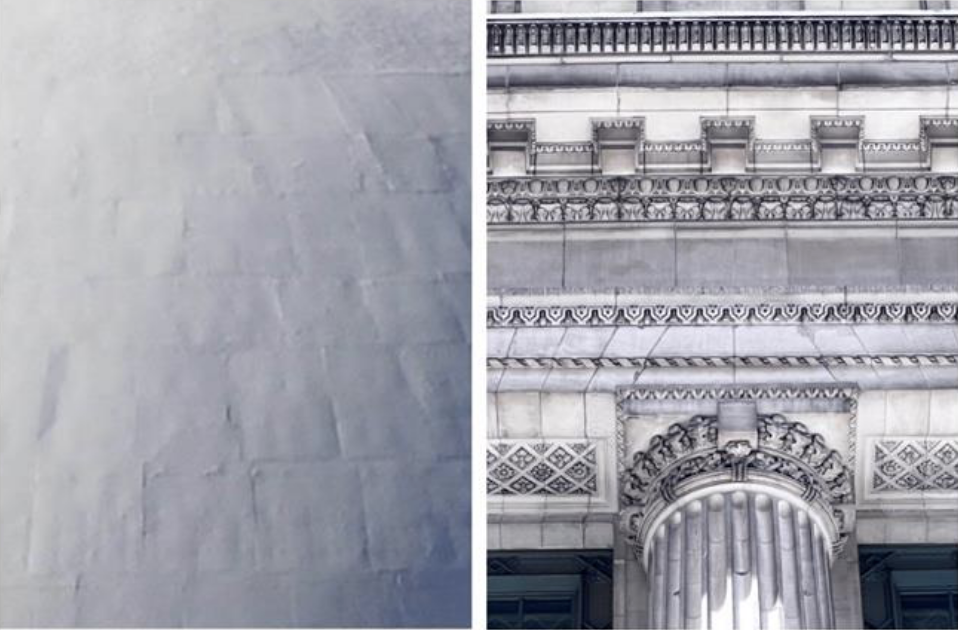
\includegraphics[height=5cm]{figures/beautyscale_image.png} }}
    \subfloat{{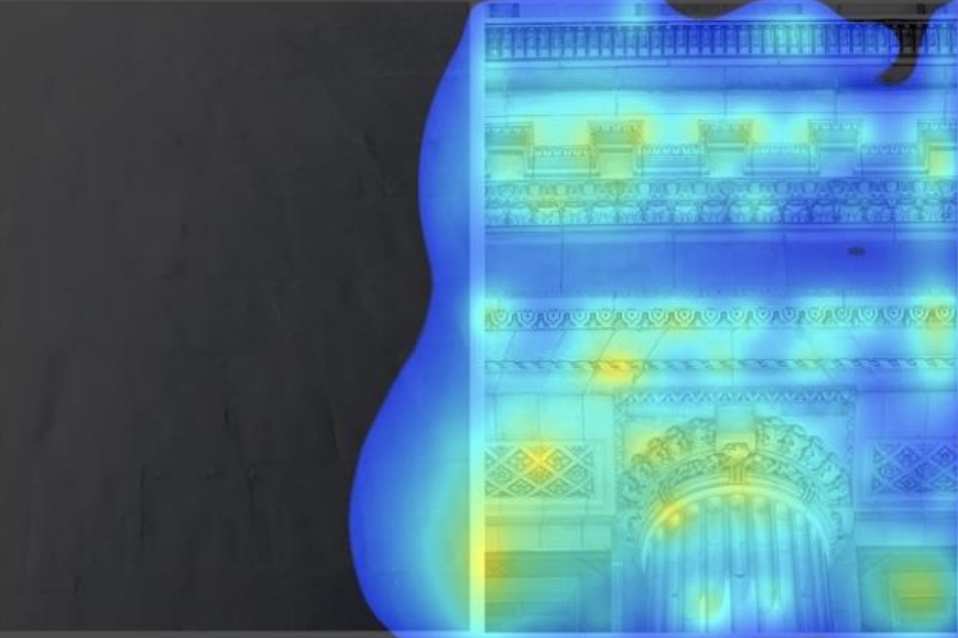
\includegraphics[height=5cm]{figures/beautyscale_heatmap.png} }}
    \caption{Left: Two designs for a building facade. Right: A heatmap reveals the degree to which the two different facade designs capture the attention of study participants. The heatmap was generated from eye-tracking data. As expected, the feature-rich pillar capital and lower-side cornice of the right facade retains visual attention to a much higher degree. Source:Figure 6 from Lavdas' and Salingaros' seminal publication \textit{"Architectural Beauty: Developing a Measurable and Objective Scale"} \cite{lavdas_architectural_2022}}
    \label{fig:heatmap}
\end{figure}

\clearpage
\section{Connecting Aesthetics and Sustainability}

Studies show that 


\clearpage
\section{Proposed Speakers}

\subsection{Day 1: History of Architecture}

Pending recommendations by Samuel Leder et al.
Ideally some scholars of art and/or architectural history.
If we can get at least \textit{one} architect here, we could avoid questions of the sort "Why don't you have any architects among the speakers?".

eg. in the example of church architecture
church architecture as case study of representative architecture
Hundertwasser - how to include him?


\subsection{Day 2: Sustainability in the Built Environment}

Pending recommendations by Romain Sacchi and Xiaojin Zhang.
I could also ask Martin Röck if he can either recommend someone or if he wants to take part himself.
Could be someone from ETH, as long as they're interesting enough.
We could do some simple LCA calculations (using Brightway Live) to show the differences between

\subsection{Day 3: Biophilic Design}



\subsection{Day 4: Measuring Aesthetics}

\subsection{Day 5: Bringing it all together...}

\subsection{Days 6-7: To be determined...}

Excursion to Milano (eg.)
More interactive content in the first days.


\begin{figure}
    \centering
    \subfloat{{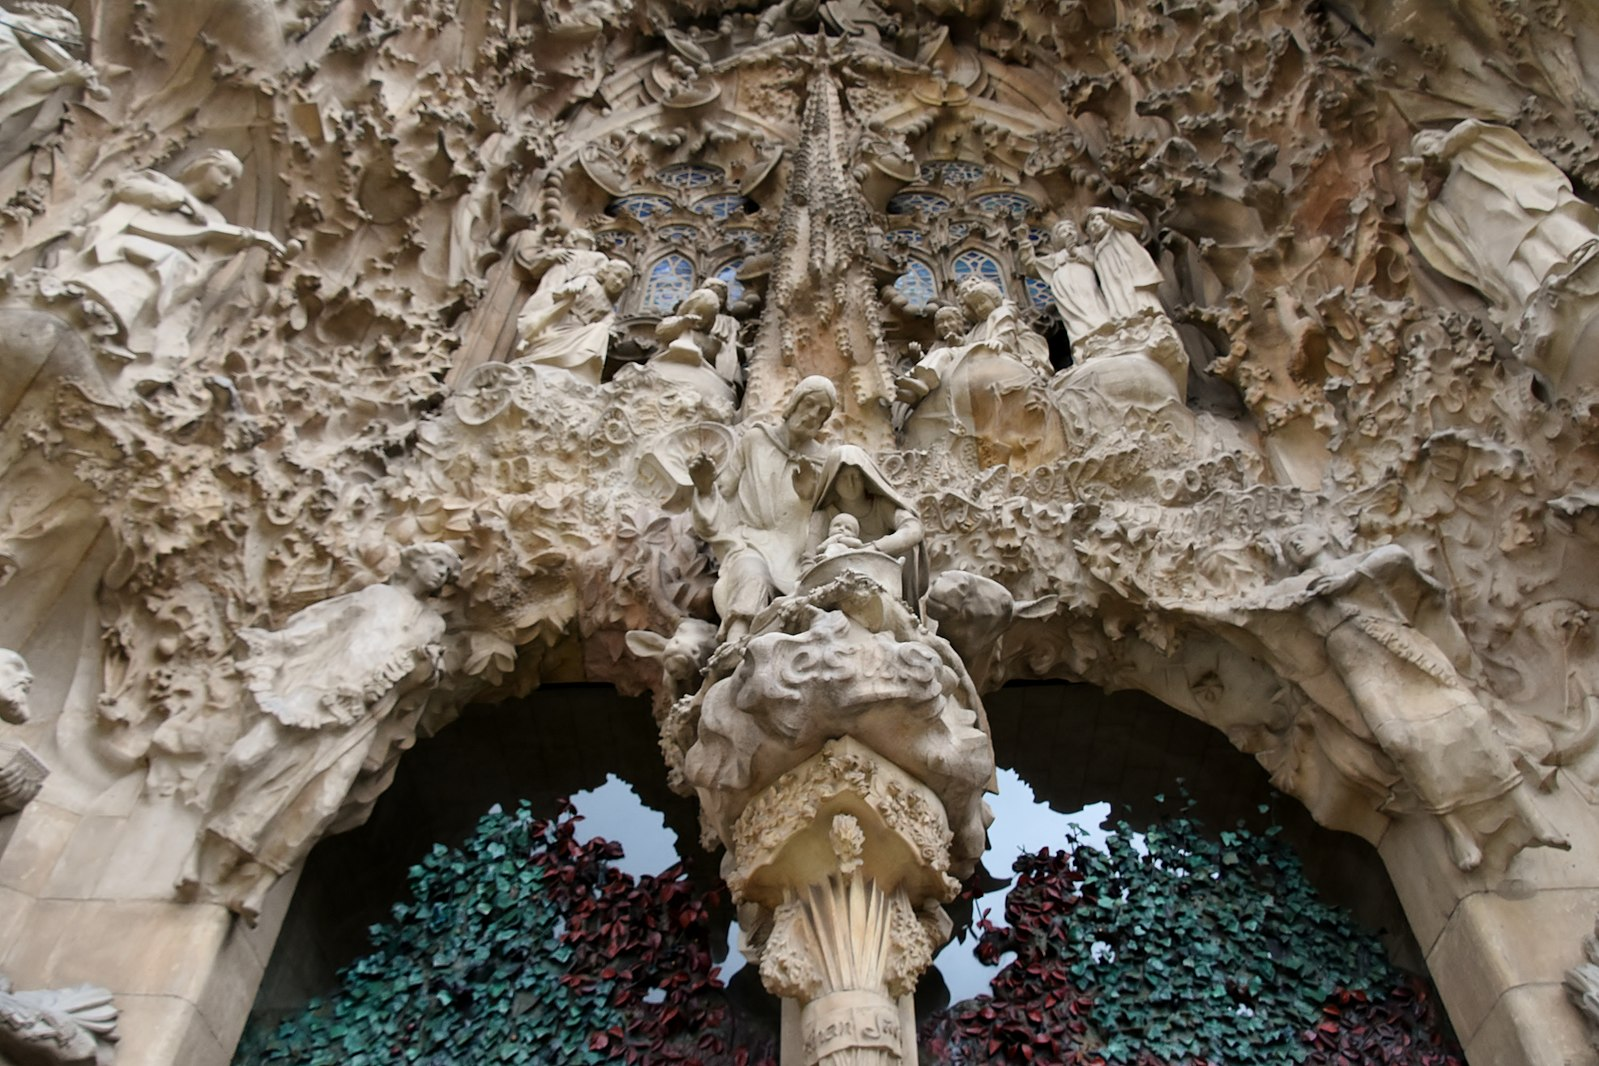
\includegraphics[height=4cm]{figures/sagrada_facade.jpg} }}
    \subfloat{{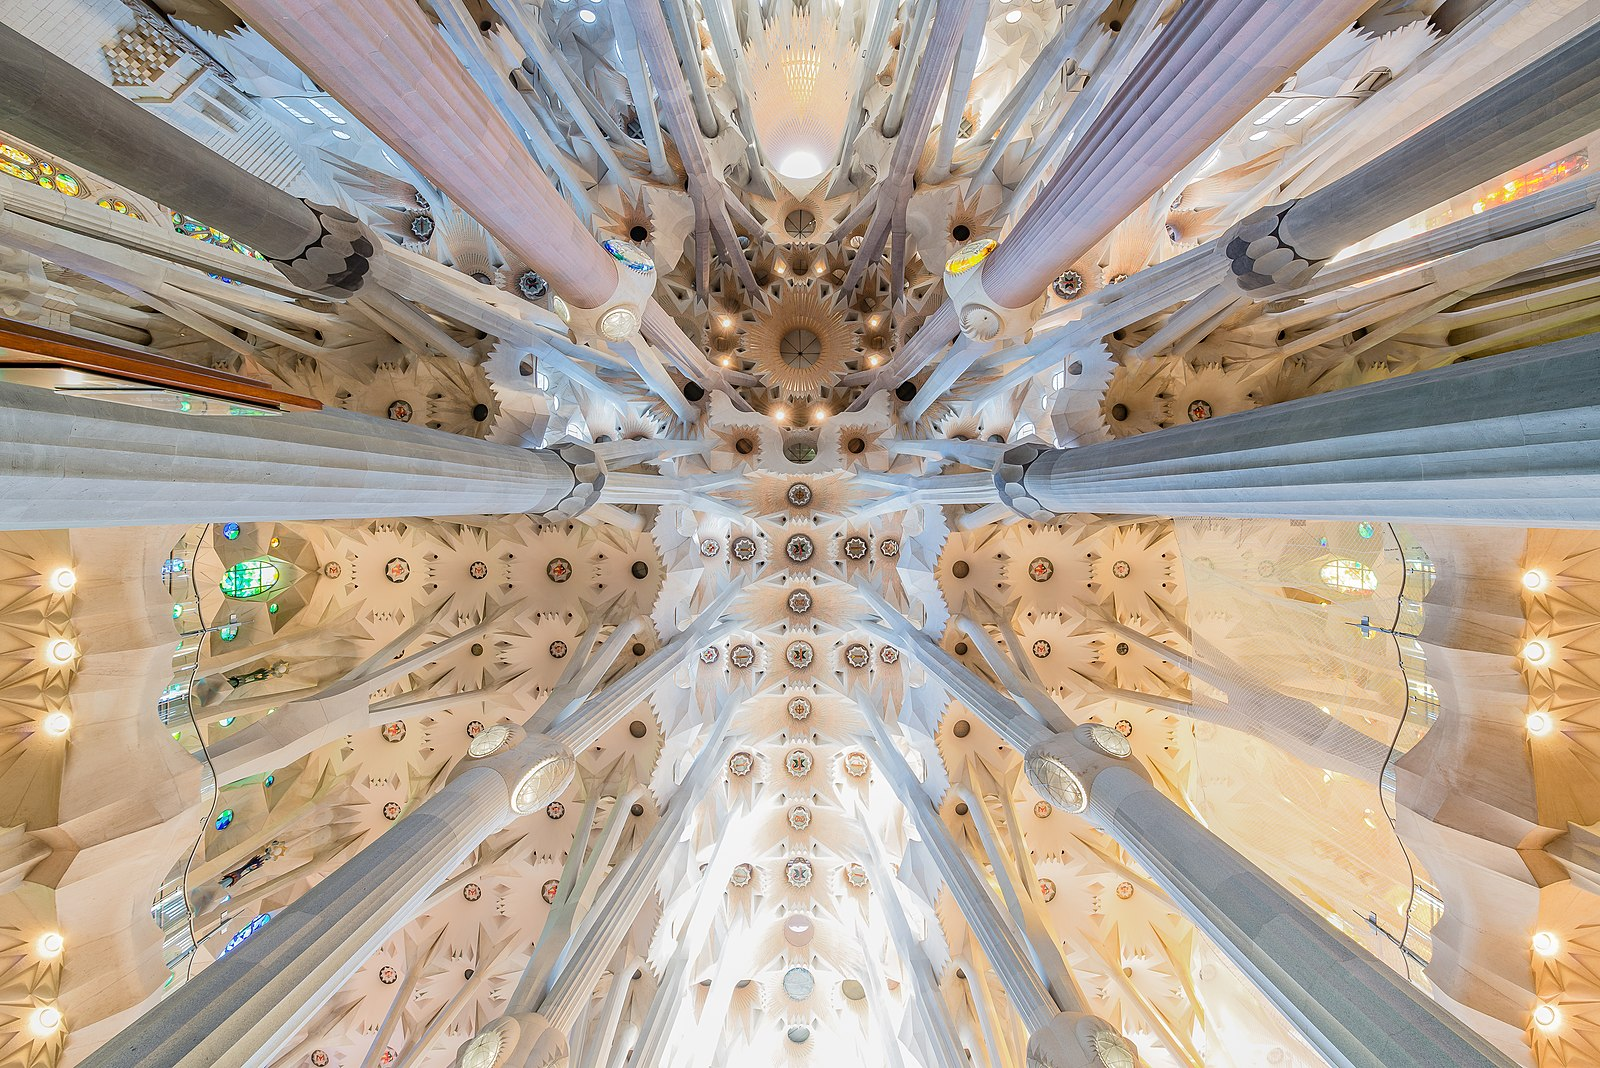
\includegraphics[height=4cm]{figures/sagrada_interior.jpg} }}
    \caption{Gothic Revival, Art Nouveau and Modernista catholic church "Sagrada Familia" (en.: "Holy Family") in Barcelona, Spain, designed by Antoni Gaudí from 1883 until his death in 1926. Left: Detail of the nativity façade with XXXX. Right: Wide-angle view of the   Image sources from left to right: Outside view \cite{mortel_sagrada_2016} and inside view \cite{wikimedia_commons_user_t_meltzer_sagrada_2014}.}
    \label{fig:kunstformen}
\end{figure}

\begin{figure}
    \centering
    \subfloat{{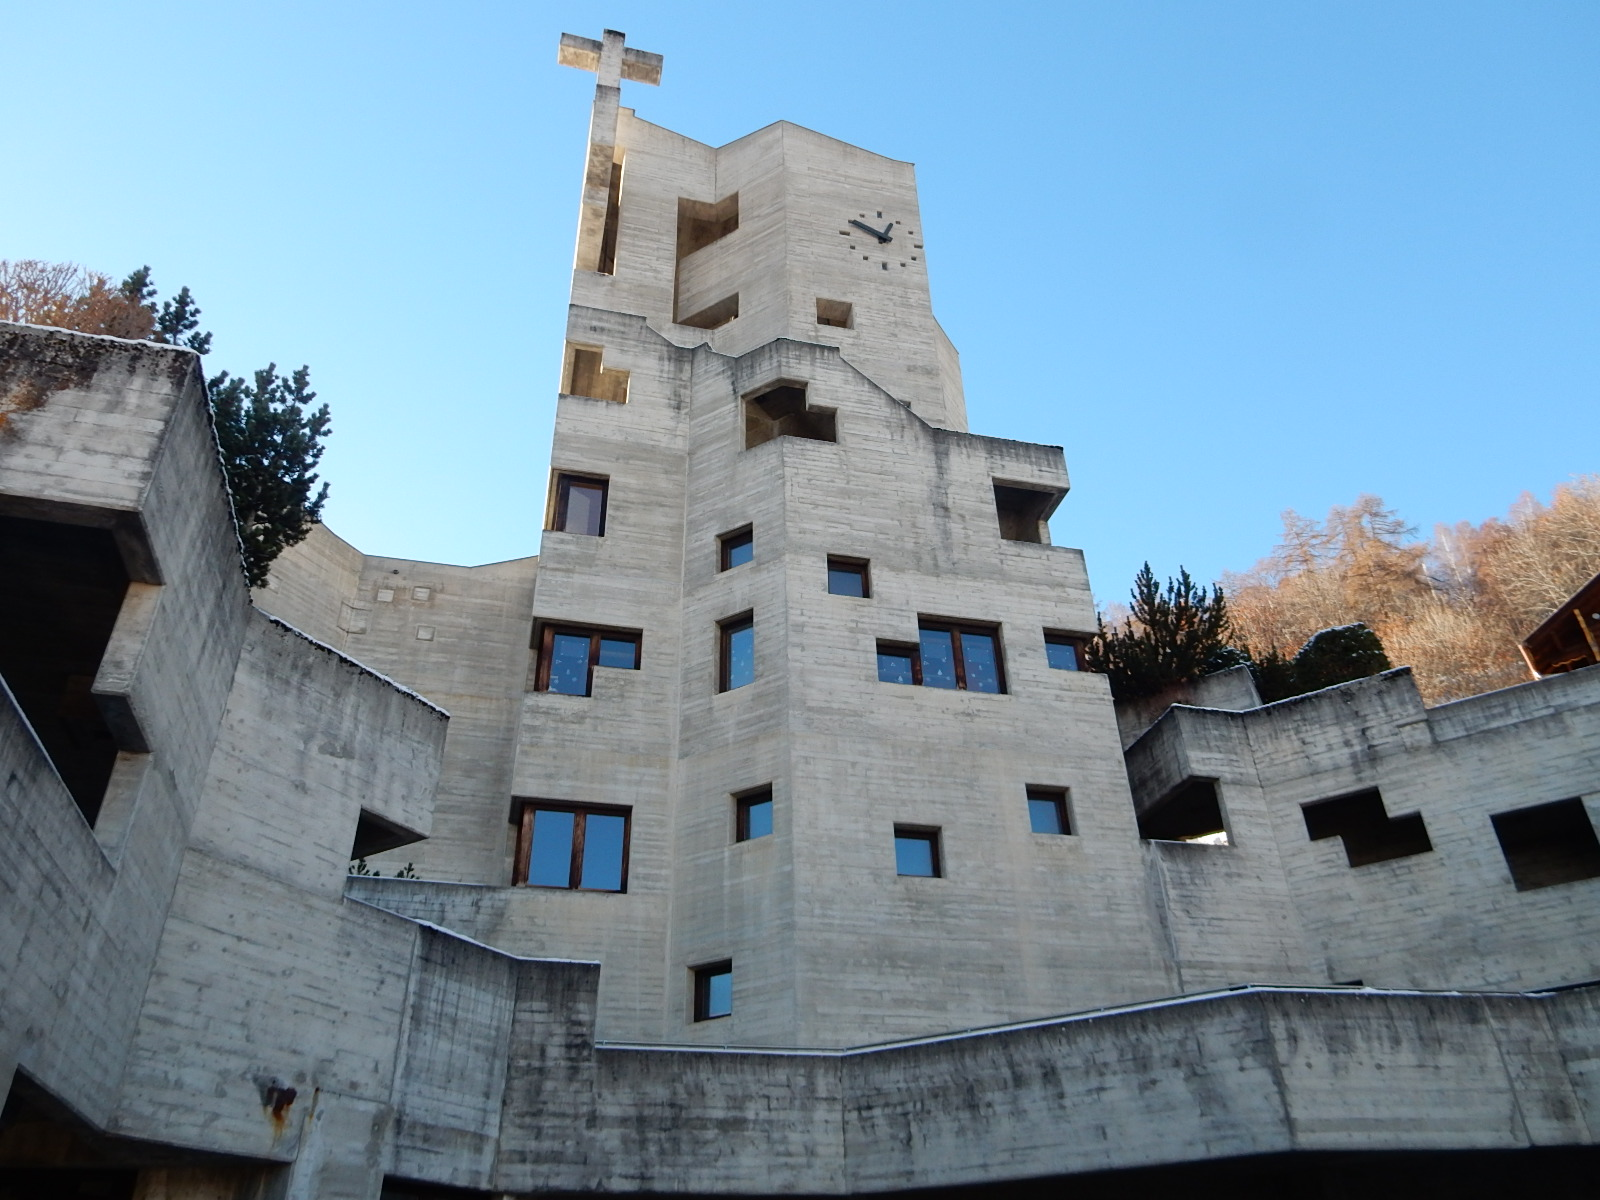
\includegraphics[height=4.5cm]{figures/hérémence_1.jpg} }}
    \subfloat{{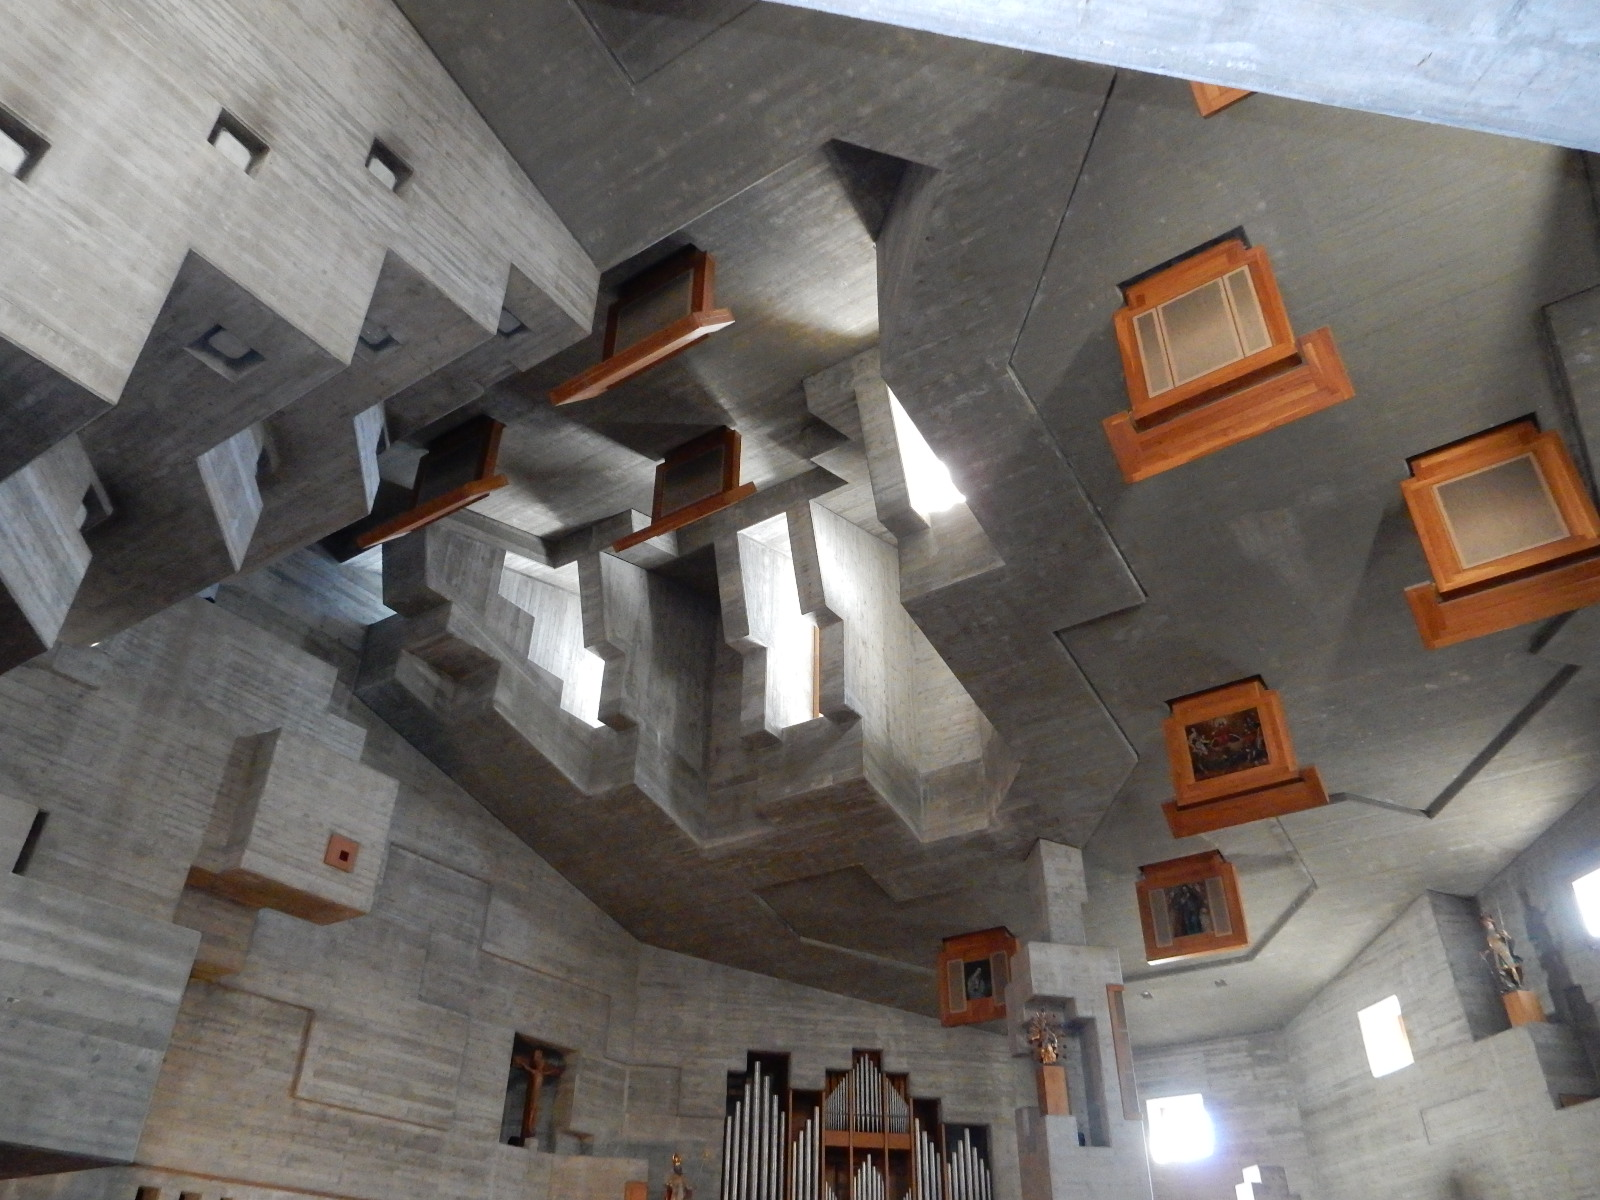
\includegraphics[height=4.5cm]{figures/hérémence_2.jpg} }}
    \caption{Brutalist-style catholic church "St. Nicolas" in the Swiss mountain village of Hérémence, designed by Walter Maria Förderer in 1967. Image sources from left to right: Outside view \cite{bissegger_eglise_2018-1} and inside view \cite{bissegger_eglise_2018}.}
    \label{fig:kunstformen}
\end{figure}

\newpage

\begin{figure}
    \centering
    \subfloat{{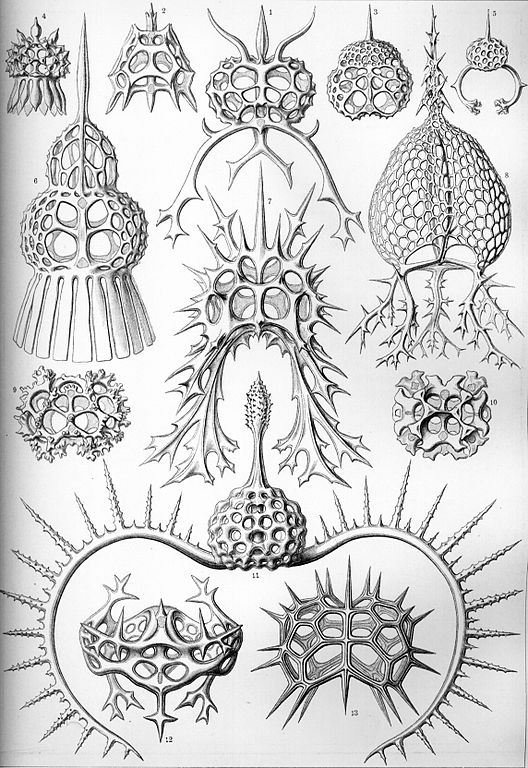
\includegraphics[height=5.5cm]{figures/Spyroidea.jpg} }}
    \subfloat{{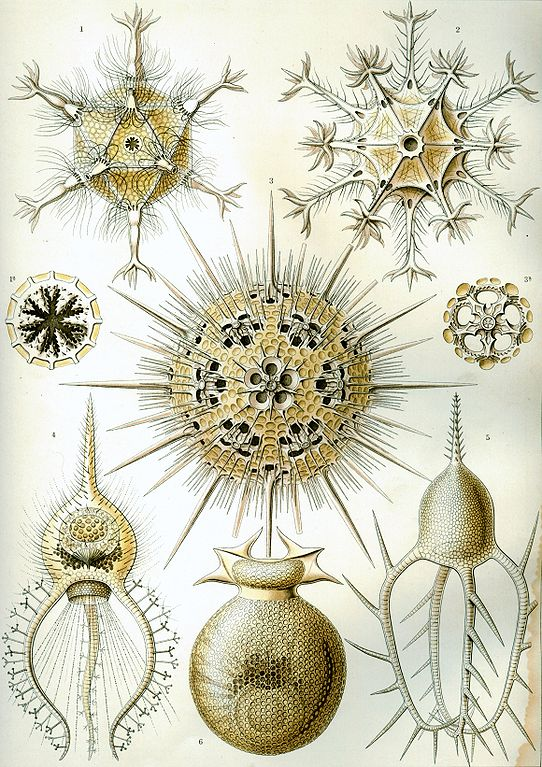
\includegraphics[height=5.5cm]{figures/Phaeodaria.jpg} }}
    \subfloat{{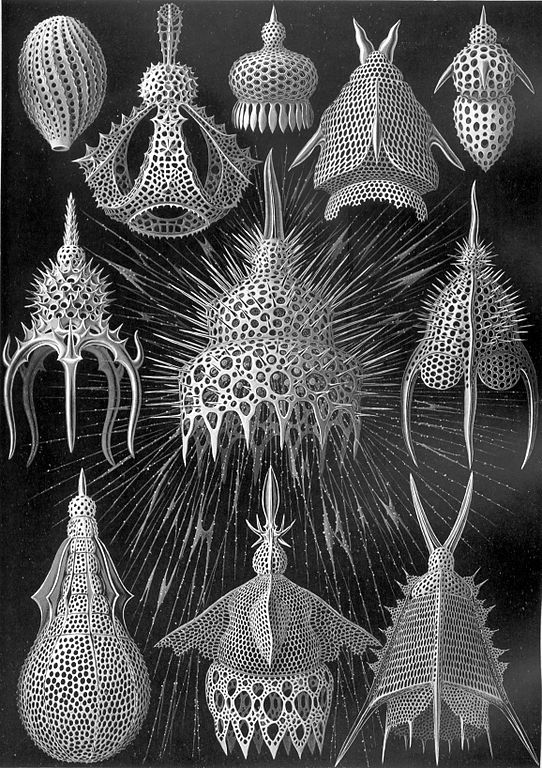
\includegraphics[height=5.5cm]{figures/Cyrtoidea.jpg} }}
    \caption{Selection of drawings from Ernst Haeckel's \textit{"Kunstformen der Natur" (en.: "Art Forms in Nature")} \cite{haeckel_kunstformen_2012}. According to Rene Binet, drawings like these served as inspiration for his monumental arch \cite[Sec. "Haeckel und der Jugendstil"]{willmann_haeckel_2019}, which is depicted in \cref{fig:arch}. Image sources from left to right: Spyroidea \cite{haeckel_kunstformen_1904}, Phaeodaria \cite{haeckel_kunstformen_1904} and Cyrtoidea \cite{haeckel_kunstformen_1904-2} by Ernst Haeckel.}
    \label{fig:kunstformen}
\end{figure}

\begin{figure}
    \centering
    \subfloat{{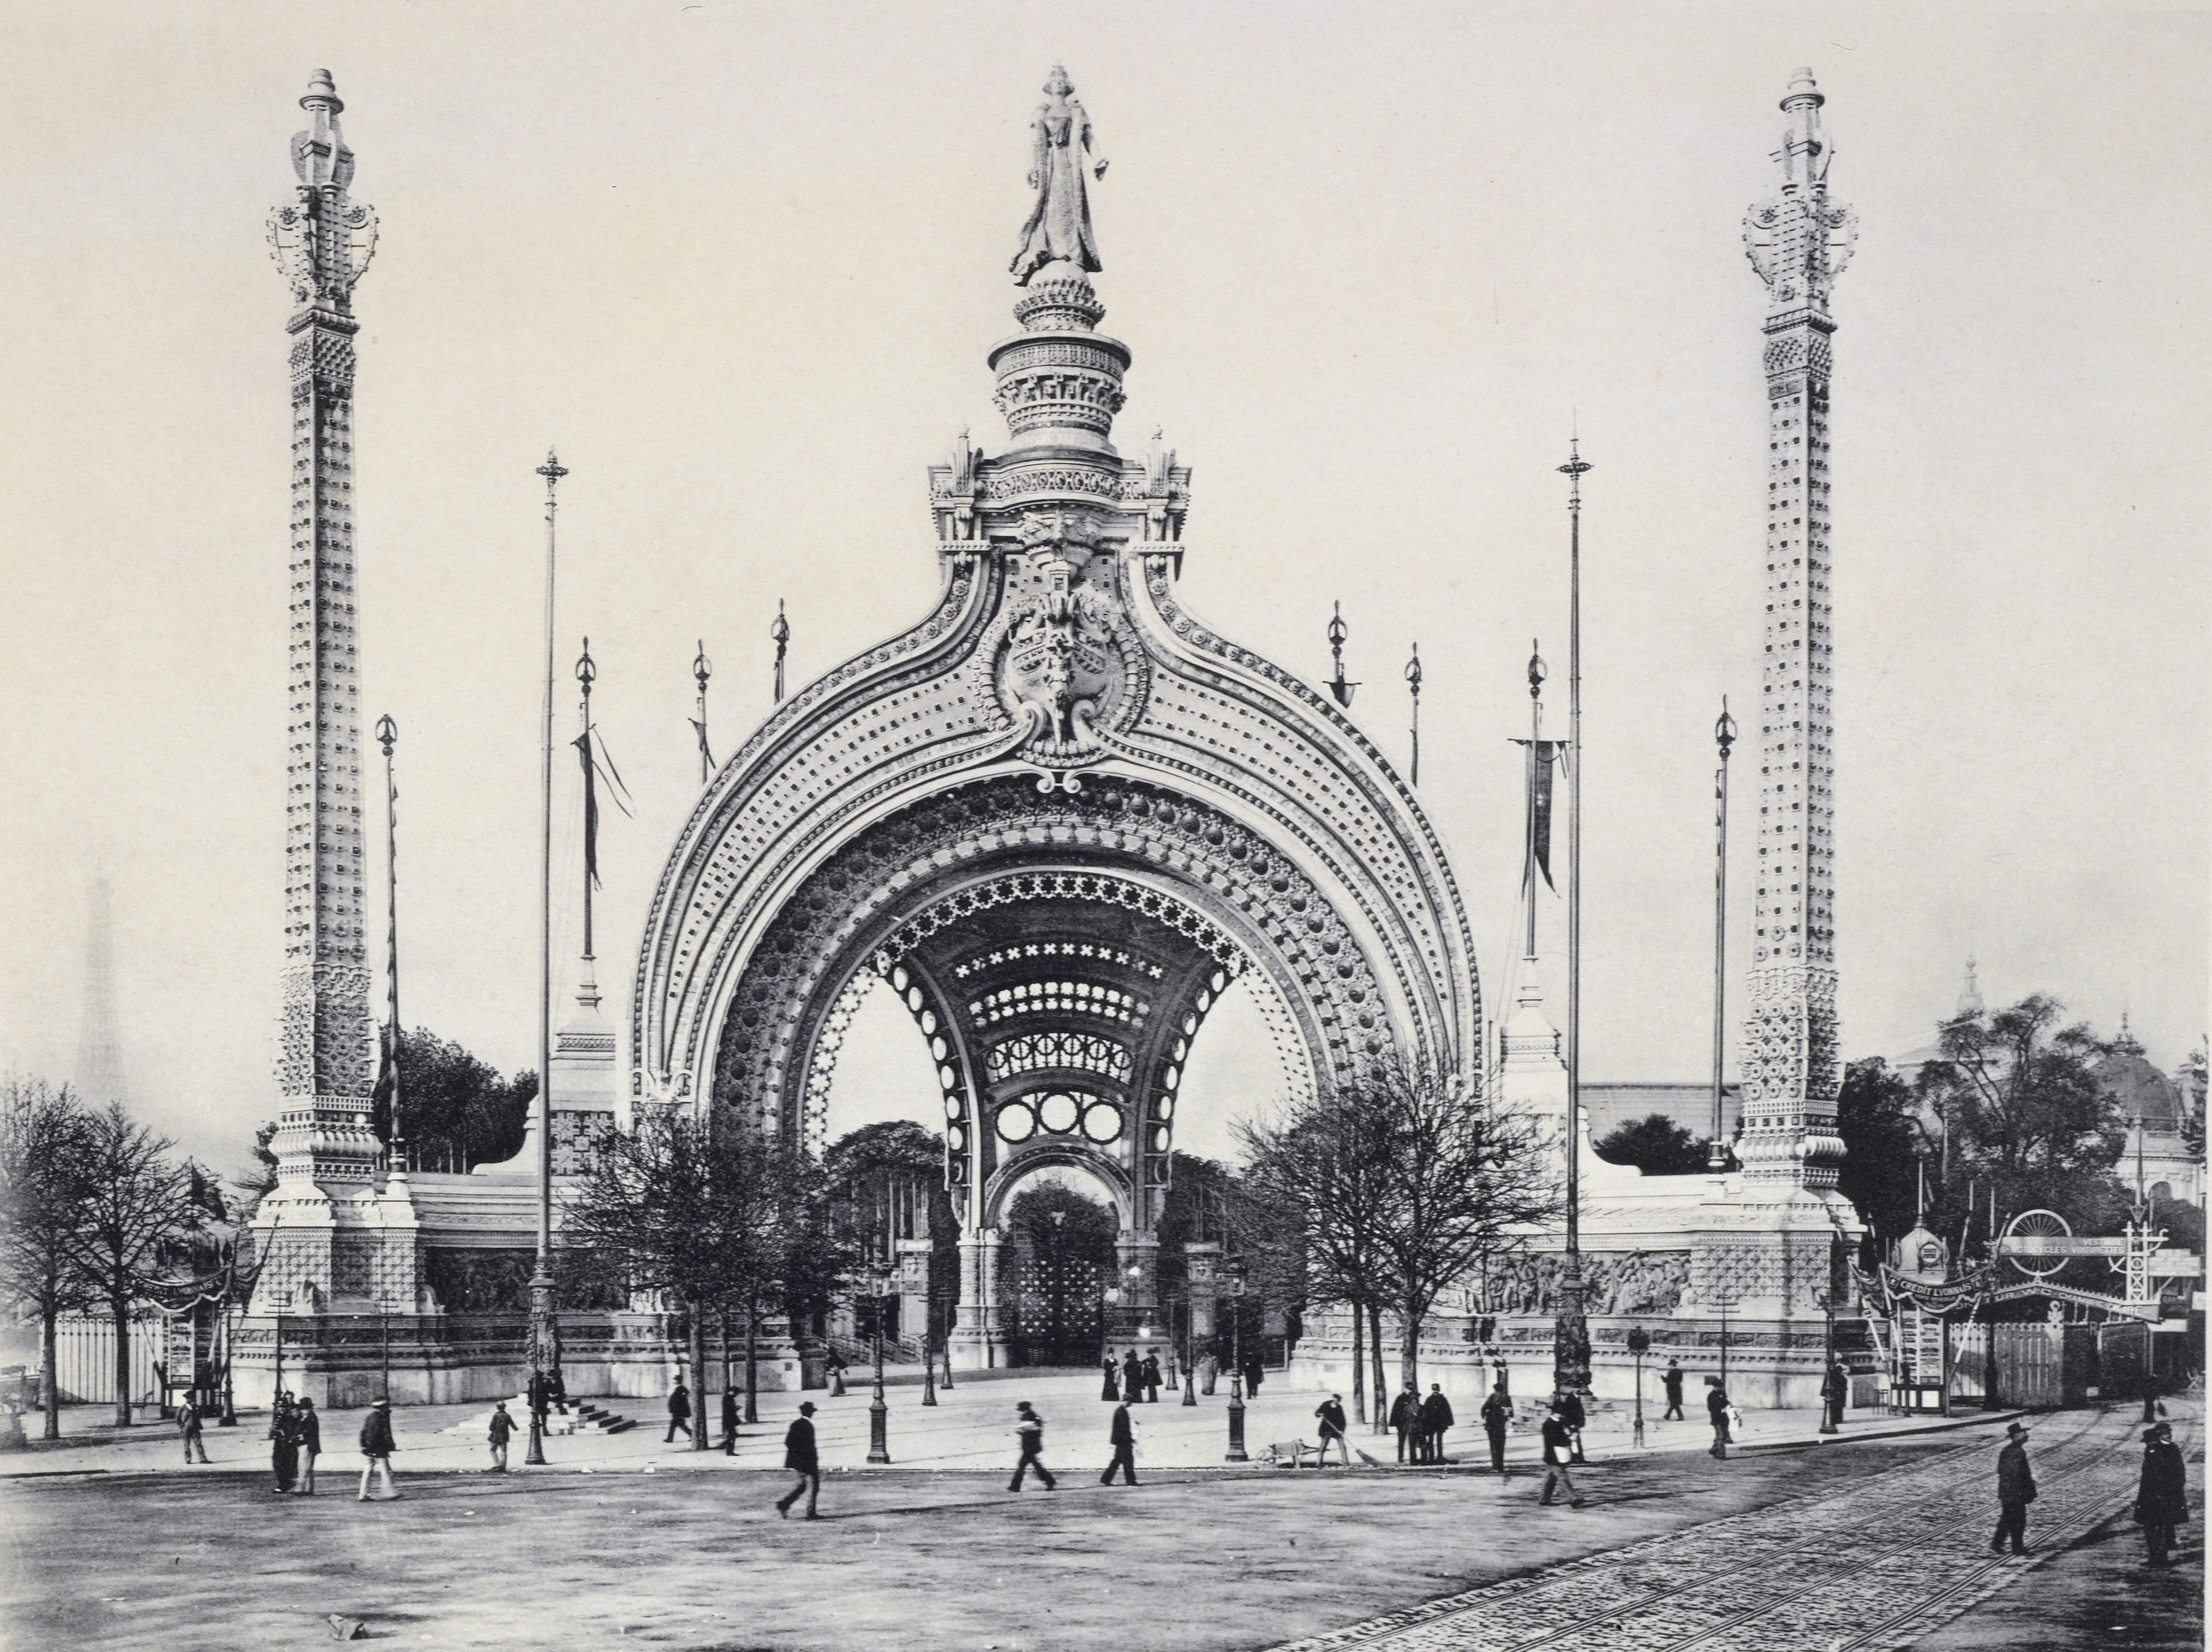
\includegraphics[height=4cm]{figures/porte_photograph.jpg} }}
    \subfloat{{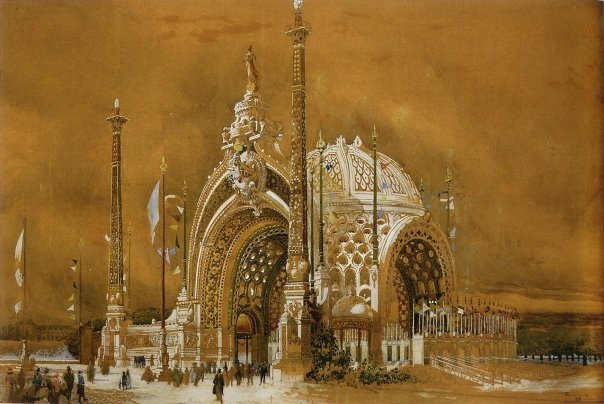
\includegraphics[height=4cm]{figures/porte_watercolor.jpg} }}
    \caption{Two renderings of the \textit{"Porte Binet"}, a monumental gate designed by Rene Binet for the 1900 Paris Exposition. Image sources: Photograph by Larger \cite{louis_porte_1900} and watercolor on paper by Binet \cite{binet_projet_1898}.}
    \label{fig:arch}
\end{figure}

\clearpage
\printbibliography

\end{document}
